\documentclass[11pt]{article}
\usepackage{enumerate}
\usepackage{fullpage}
\usepackage{fancyhdr}
\usepackage{amsmath, amsfonts, amsthm, amssymb}
\usepackage{color}
\usepackage{graphicx}
\setlength{\parindent}{0pt}
\setlength{\parskip}{5pt plus 1pt}
\pagestyle{empty}

\def\indented#1{\list{}{}\item[]}
\let\indented=\endlist

\newcounter{questionCounter}
\newcounter{partCounter}[questionCounter]
\newenvironment{question}[2][\arabic{questionCounter}]{%
    \setcounter{partCounter}{0}%
    \vspace{.25in} \hrule \vspace{0.5em}%
        \noindent{\bf #2}%
    \vspace{0.8em} \hrule \vspace{.10in}%
}{}

%%%%%%%%%%%%%%%%%%%%%%%HEADER%%%%%%%%%%%%%%%%%%%%%%%%%%%%%%
\newcommand{\myname}{Shashank Singh}
\newcommand{\myandrew}{sss1@andrew.cmu.edu}
\newcommand{\myclass}{10-601 Machine Learning}
\newcommand{\myhwnum}{2}
\newcommand{\duedate}{Friday, September 28, 2012}
%%%%%%%%%%%%%%%%%%%%%%%%%%%%%%%%%%%%%%%%%%%%%%%%%%%%%%%%%%%

%%%%%%%%%%%%%%%%%%%%CONTENT MACROS%%%%%%%%%%%%%%%%%%%%%%%%%
\renewcommand{\qed}{\quad $\blacksquare$}
\newcommand{\mqed}{\quad \blacksquare}
\newcommand{\inv}{^{-1}}
\newcommand{\bw}{\mathbf{w}}
\newcommand{\by}{\mathbf{y}}
\newcommand{\bff}{\mathbf{f}}
\newcommand{\bzero}{\mathbf{0}}
\newcommand{\bxi}{\boldsymbol{\xi}}
\newcommand{\boldeta}{\boldsymbol{\eta}}
\newcommand{\pr}[1]{\mathsf{P}\left( #1 \right)} % probability of event #1
\newcommand{\Bern}[1]{\operatorname{Bernoulli}\left( #1 \right)} % Bernoulli distribution of parameter p
\newcommand{\argmax}{\operatorname{argmax}}
\newcommand{\N}{\mathbb{N}} % natural numbers
\newcommand{\Q}{\mathbb{Q}} % rational numbers
\newcommand{\R}{\mathbb{R}} % real numbers
%%%%%%%%%%%%%%%%%%%%%%%%%%%%%%%%%%%%%%%%%%%%%%%%%%%%%%%%%%%

\begin{document}
\thispagestyle{plain}

{\Large Homework \myhwnum} \\
\myclass \\
Name: \myname \\
Email: \myandrew \\
Due: \duedate \\

\section{Naive Bayes}
\subsection*{Problem 1. Basic Concepts.}
\begin{enumerate}[a.]
\item Yes;
\[\pr{X,Y | Z} = \pr{X | Y,Z} \cdot \pr{Y | Z} = \pr{X | Z} \cdot \pr{Y | Z}.\]

\item Suppose $X = Y = Z$, where $Z \sim \Bern{\tfrac12}$. Then,
$\pr{X | Y,Z} = \pr{X | Z}$, but
\[\pr{X = 1, Y = 1} = \tfrac12 \neq \tfrac14 = \pr{X = 1} \cdot \pr{Y = 1}.\]

\item Since no $\theta_{ij}$ parameter can be determined from any subset of
the other $\theta_{ij}$ parameters, there are \fbox{$nJ$} independent
$\theta_{ij}$ parameters.

\item Since no $\mu_{ij}$ or $\sigma_{ij}$ parameter can be determined from
any subset of the other $\mu_{ij}$ or $\sigma_{ij}$ parameters, there are
\fbox{$2nJ$} independent $\mu_{ij}$ or $\sigma_{ij}$ parameters.

\item Since the term $\sum_j \pr{Y = y_j} \prod_i \pr{X_i | Y = y_j}$ does not
depend on $y_k$,
\[y^*
 = \argmax_{y_k} \frac{\pr{y = y_k} \prod_i \pr{x_i | y = y_k}}
           {\sum_j \pr{Y = y_j} \prod_i \pr{X_i | Y = y_j}}
 = \argmax_{y_k} \pr{y = y_k} \prod_i \pr{x_i | y = y_k}.
\]

\item Yes; since Naive Bayes is a generative classifier, an estimates of
$\pr{X}$ can be computed from the parameters estimated by Naive Bayes using
Bayes Rule.
\end{enumerate}

\subsection*{Problem 2. Parameter estimation for Naive Bayes}
\begin{enumerate}[a.]
\item
\[\operatorname{MLE}(\hat{\theta}_{1k})
 = \mbox{\fbox{$\displaystyle \frac{\sum_{j = 1}^M x_{1j}}{M}$.}}\]

\item Since the training instances are independent,
\[P(X | Y)
 = \prod_{j = 1}^M P(X_j | Y_j).\]

Thus,
\begin{align*}
\operatorname{MLE}(\mu_{ik})
 & = \argmax_{\mu \in \R} \ln \left( \prod_{j = 1}^M \frac{1}{\sigma_{ik}\sqrt{2\pi}}\exp\left( \frac{-(x_{ij} - \mu_{ik})^2}{2\sigma_{ik}^2} \right) \right) \\
 & = \argmax_{\mu \in \R} \sum_{j = 1}^M \ln \left( \frac{1}{\sigma_{ik}\sqrt{2\pi}}\exp\left( \frac{-(x_{ij} - \mu_{ik})^2}{2\sigma_{ik}^2} \right) \right) \\
 & = \argmax_{\mu \in \R} \sum_{j = 1}^M \ln \left( \exp\left( -(x_{ij} - \mu_{ik})^2 \right) \right) \\
 & = \argmax_{\mu \in \R} \sum_{j = 1}^M -(x_{ij} - \mu_{ik})^2.
\end{align*}
Therefore, $\mu_{ik}$ is the value which minimizes the sum of squared errors
of the $x_{ij}$ values, so that \[\mu_{ik} = \mbox{\fbox{$\displaystyle \frac{\sum_{j = 1}^M x_{ij}}{M}$,}}\]
the mean of the $x_{ij}$ values.
\end{enumerate}

\section{Regularized Multi-Class Logistic Regression}
\begin{enumerate}[a.]
\item If we let $\bw_K = 0$, then, since $\exp(0) = 1$,
\begin{align*}
L(\bw_1,\dots,\bw_K)
 & = \ln \left( \prod_{l = 1}^D \pr{Y^l | X^l,W} \right) - \sum_{k = 1}^K \frac{\lambda}{2}\|\bw_k\|^2 \\
 & = \sum_{l = 1}^D \ln(\pr{Y^l | X^l,W}) - \sum_{k = 1}^K \frac{\lambda}{2}\|\bw_k\|^2 \\
 & =                      \ln\left( \frac{1}{1 + \sum_{t = 1}^{K - 1}\exp(\bw_t \cdot x_t)} \right) \\
 & + \sum_{l = 1}^D \ln\left( \frac{\exp(\bw_k \cdot x_k)}{1 + \sum_{t = 1}^{K - 1}\exp(\bw_t \cdot x_t)} \right) - \sum_{k = 1}^K \frac{\lambda}{2}\|\bw_k\|^2 \\
 & = \sum_{l = 1}^D \ln\left( \frac{\exp(\bw_k \cdot x_k)}{\sum_{t = 1}^{K - 1}\exp(\bw_t \cdot x_t)} \right) - \sum_{k = 1}^K \frac{\lambda}{2}\|\bw_k\|^2 \\
 & = \sum_{l = 1}^D \bw_{Y^l} \cdot x_k - \ln \left[ \sum_{t = 1}^K\exp(\bw_t \cdot x_t)\right] - \sum_{k = 1}^K \frac{\lambda}{2}\|\bw_k\|^2.
\end{align*}

%TODO
\item Differentiating the above expression with respect to $w_{ij}$ gives
\begin{align*}
\frac{\partial L(\bw_1,\dots,\bw_K)}{\partial w_{ij}}
 & = \frac{\partial}{\partial w_{ij}}
 \sum_{l = 1}^D \bw_{Y^l} \cdot x_k - \ln \left[ \sum_{t = 1}^K\exp(\bw_t \cdot x_t)\right] - \sum_{k = 1}^K \frac{\lambda}{2}\|\bw_k\|^2. \\
 & = \sum_{l = 1}^D \delta(Y^l = k)x_k^l) - \left[\frac{\partial}{\partial w_{ij}} \ln \left[ \sum_{t = 1}^K\exp(\bw_t \cdot x_t)\right]\right] - \lambda w_{ij} \\
 & = \left(\sum_{l - 1}^D X_i^l\left(\delta(Y^l = k) - \pr{Y^l = k | X^l,\bw_1,\dots,\bw_k} \right) \right) - \lambda w_{ki}.
\end{align*}
where $\delta(Y^l = k)$ is $1$ if $Y^l = k$ and $0$ otherwise.

Thus, the desired gradient is
\[\frac{\partial L(\bw_1,\dots,\bw_K)}{\partial \bw_i}
 = \begin{bmatrix}
     \frac{\partial L(\bw_1,\dots,\bw_K)}{\partial w_{i1}} \\
     \frac{\partial L(\bw_1,\dots,\bw_K)}{\partial w_{i2}} \\
     \vdots                                                \\
     \frac{\partial L(\bw_1,\dots,\bw_K)}{\partial w_{iK}} \\
   \end{bmatrix}
\]

\item The update rule is
\[w_{ki}
  \leftarrow w_{ki}
  +          \nu \left(\sum_{l - 1}^D X_i^l\left(\delta(Y^l = k)
                        - \pr{Y^l = k | X^l,\bw_1,\dots,\bw_k} \right) \right)
  - \nu\lambda w_{ki}.
\]

\item Since the log likelihood function is concave in each $\bw_i$, it is
concave in $(\bw_1,\dots,\bw_k)$, so that the gradient ascent will converge
on a global maximum.

\end{enumerate}

\section{Generative-Discriminative Classifiers}
\begin{enumerate}[a.]
%TODO
\item By Bayes Rule and the Law of Total Probability,
\begin{align*}
\pr{Y = 1 | X}
 & = \frac{\pr{Y = 1} \cdot \pr{X | Y = 1}}
        {\pr{Y = 1} \cdot \pr{X | Y = 1} + \pr{Y = 0} \cdot \pr{X | Y = 0}} \\
 & = \frac{1}
        {1 + \frac{\pr{Y = 0} \cdot \pr{X | Y = 0}}
                  {\pr{Y = 1} \cdot \pr{X | Y = 1}}}
   = \frac{1}
        {1 + \exp\ln\frac{\pr{Y = 0} \cdot \pr{X | Y = 0}}
                  {\pr{Y = 1} \cdot \pr{X | Y = 1}}}                        \\
 & = \frac{1}
        {1 + \exp\left(          \ln \frac{\pr{Y = 0}}
                                          {\pr{Y = 1}}
                + \sum_{i = 1}^n \ln \frac{\pr{X_i | Y = 0}}
                                          {\pr{X_1 | Y = 1}}
                 \right)}                                                   \\
 & = \frac{1}
        {1 + \exp\left(          \ln \frac{1 - \pi}
                                          {\pi}
                + \sum_{i = 1}^n \ln \frac{\pr{X_i | Y = 0}}
                                          {\pr{X_i | Y = 1}}
                 \right)}                                                   \\
\end{align*}
where $\pi := \pr{Y = 1}$. Letting $\theta_{ik} := \pr{X_i = 1 | Y = k}$ (for
$k \in \{0,1\}$),
\begin{align*}
\sum_{i = 1}^n \ln \frac{\pr{X_i | Y = 0}}{\pr{X_i | Y = 1}}
 & = \sum_{i = 1}^n  \ln \frac{\theta_{i0}^{X_i}(1 - \theta_{i0})^{1 - X_i}}
              {\theta_{i1}^{X_i}(1 - \theta_{i1})^{1 - X_i}}                \\
 & = \sum_{i = 1}^n \left( \ln \frac{\theta_{i0}(1 - \theta_{i1})}
                     {\theta_{i1}(1 - \theta_{i0})}  \right) X_i
   + \ln \frac{(1 - \theta_{i0})}{(1 - \theta_{i1})}.                       \\
\end{align*}
Thus, for
\[w_0 = \ln \frac{1 - \pi}{\pi}
  + \sum_{i = 1}^n \ln \left( \frac{1 - \theta_{i0}}{1 - \theta_{i1}} \right)
   \quad \mbox{ and } \quad
  w_i = \left( \ln \frac{\theta_{i0}(1 - \theta_{i1})}
                      {\theta_{i1}(1 - \theta_{i0})} \right)
         \mbox{ (for $i \in \{1,2,\dots,n\}$),}
\]

\[\pr{Y = 1 | X}
 = \frac{1}{1 + \exp \left( w_0 + \sum_{i = 1}^n w_iX_i\right)},\]
which is the desired logistic form. \qed

\item When the conditional independence assumption holds, Naive Bayes and
Logistic Regression are equivalent, so neither produces better results.

\item Since Naive Bayes depends on the assumption that
$\pr{X_i | Y,X_j} = \pr{X_i | X}$ to simplify the parameters it must estimate,
it is less accurate than logistic regression when this assumption does not
hold.

\item No; since Logistic Regression is a discriminative classifier, it cannot
estimate $\pr{X}$.

\end{enumerate}

\section{Programming}
\subsection*{4.1 Feature selection with Mutual Information}
\begin{enumerate}[a.]
\item

\begin{tabular}{|r|c|c|c|}
  \hline
  Classifer             & Training Accuracy & Testing Accuracy & Training Time      \\
  \hline
  Logistic Regression   & 0.9918            & 0.9878           &  $0.1414$ seconds  \\
  \hline
  Naive Bayes           & 0.9901            & 0.9834           &  $0.0891$ seconds  \\
  \hline
\end{tabular}

\begin{figure}[h]
\begin{center}
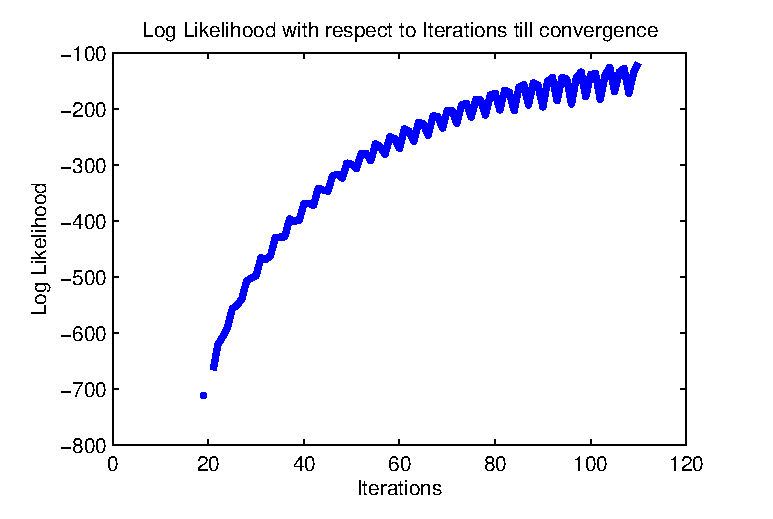
\includegraphics[width=0.46\textwidth]{4}
\end{center}
\label{fig:1}
\end{figure}
\end{enumerate}

\end{document}
